%!TEX root = ../thesis.tex

\section{ネットワーク構造}
提案手法で用いた学習器のネットワークを\figref{Fig:network_structure}に示す. また, ハイパーパラメータについてtableに示す. 64x48のRGB画像を入力とする入力層1層, 畳み込み層3層, 全結合層2層を持つ6層のCNNと, このCNNの出力と目標方向指令を入力する入力層1層, 全結合層2層, 出力層1層の全10層から構成されている. 出力はヨー方向の角速度である.

\begin{figure}[hbtp]
  \centering
 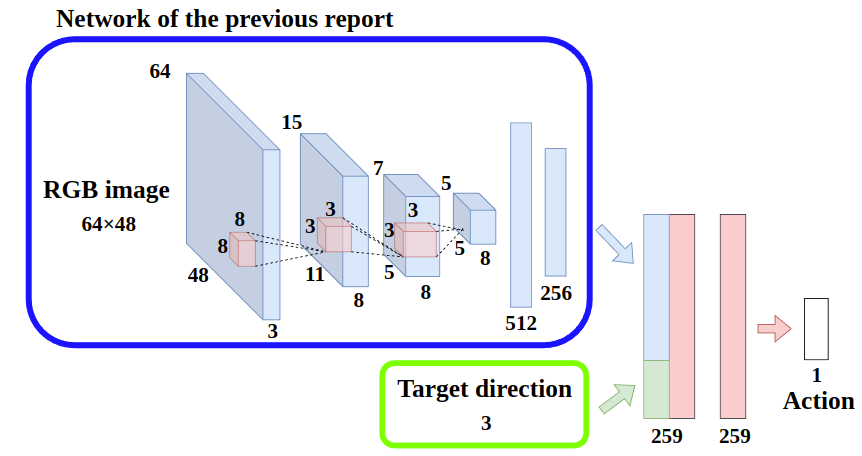
\includegraphics[keepaspectratio, scale=0.43]
      {images/network_structure2.png}
 \caption{Method network}
 \label{Fig:network_structure}
\end{figure}

\begin{table}[hbtp]
  \caption{Parameters of network}
  \label{table:param1}
  \centering
  \begin{tabular}{|c|c|}
    \hline
    Input data & Image(64x48 pixels, RGB channels), Target direction \\
    \hline
    Optimizer & Adam($alpha = 0.001, beta1 = 0.9, beta2 =  0.999, eps = 1e^{-2}$)\\
    \hline
    Loss function & Softmax-cross-entropy\\
    \hline
    Output data & Angular velocity\\
    \hline
  \end{tabular}
\end{table}

% \begin{figure}[hbtp]
%   \centering
%  \includegraphics[keepaspectratio, scale=0.45]
%       {images/network_structure.png}
%  \caption{Learning phase system of proposed method}
%  \label{Fig:network_structure}
% \end{figure}

% \subsubsection{etc...}
\newpage
